\documentclass[10pt,a4paper]{article}

\usepackage[english]{babel}
\usepackage[a4paper, left=2cm, right=2cm, top=2cm, bottom=1.62cm]{geometry}
\usepackage{amsmath}
\usepackage{multicol}
\usepackage{graphicx}
\usepackage{float}
\usepackage{booktabs}
\usepackage{caption}
\captionsetup{font=footnotesize}

\usepackage[round]{natbib}
\bibliographystyle{abbrvnat}

\usepackage{fancyhdr}
\pagestyle{fancy}
\fancyhead[L]{02460-2026 Mini-project 3}
\fancyhead[R]{s224766, s224750, s224175 \& s224233}

% For including code
% From https://www.overleaf.com/learn/latex/Code_listing
\usepackage{listings}
\usepackage{xcolor}

\definecolor{codegreen}{rgb}{0,0.6,0}
\definecolor{codegray}{rgb}{0.5,0.5,0.5}
\definecolor{codepurple}{rgb}{0.58,0,0.82}
\definecolor{backcolour}{rgb}{0.95,0.95,0.92}

\lstdefinestyle{mystyle}{
    backgroundcolor=\color{backcolour},   
    commentstyle=\color{codegreen},
    keywordstyle=\color{magenta},
    numberstyle=\tiny\color{codegray},
    stringstyle=\color{codepurple},
    basicstyle=\ttfamily\footnotesize,
    breakatwhitespace=false,         
    breaklines=true,                 
    captionpos=b,                    
    keepspaces=true,                 
    numbers=left,                    
    numbersep=5pt,                  
    showspaces=false,                
    showstringspaces=false,
    showtabs=false,                  
    tabsize=2,
    upquote=true
}

\lstset{language=Python, style=mystyle}

\begin{document}

%%% Main text part %%%

\section*{Mini-project 3 in Advanced Machine Learning (02460)}
by Frederik Svane (s224766), Marcus Christoffersen (s224750), \\
Nicholas Larsen (s224175) \& Thor H{\o}jhus (s224233) on 29 April 2026

\begin{multicols}{2}
\subsection*{Model}
We model MUTAG adjacency matrices \citep{debnath1991mutag} with a node-latent variational graph autoencoder \citep{kingma2014vae,kipf2016vgae}. The encoder maps the seven atom labels to hidden states and applies four rounds of sum-aggregation message passing:
\[
h_i^{r+1}=h_i^r+u_r\!\left(\sum_{j\in\mathcal N(i)} m_r(h_j^r)\right),
\]
where $m_r$ and $u_r$ are ReLU MLPs. Linear heads give $(\mu_i,\log\sigma_i^2)$ and $q_\phi(Z\mid X,A)=\prod_i \mathcal N(z_i;\mu_i,\operatorname{diag}\sigma_i^2)$. The decoder is an inner-product link model,
\[
p_\theta(A_{ij}=1\mid Z)=\sigma(z_i^\top z_j+b),\qquad i<j,
\]
and samples graphs by drawing $N$ from the empirical training-size distribution, $z_i\sim\mathcal N(0,I)$, Bernoulli upper-triangle edges, and symmetrizing. Training minimizes
\[
\mathcal L=\operatorname{BCE}_w(A,\hat A)+\beta\,D_{\mathrm{KL}}(q_\phi(Z\mid X,A)\Vert p(Z)),
\]
excluding padded nodes and self-loops. We used $d_h=64$, $d_z=16$, $\beta\leq0.1$ with 100-epoch warmup, Adam at $10^{-3}$, learning-rate decay $0.995$, 500 epochs, and positive-edge reweighting $w_+ = (\text{non-edges})/(\text{edges}) \approx 11$ for sparsity; at sampling we subtract $\log(w_+)$ from logits to undo the density shift from this weighting.

\subsection*{Baseline and evaluation}
The baseline is the required Erd\H{o}s--R\'enyi model \citep{erdos1959random}: sample $N$ empirically, estimate $r_N$ from all training graphs with that $N$, then draw $G(N,r_N)$. For each model we generated 1000 graphs. Novelty and uniqueness use NetworkX Weisfeiler--Lehman hashes \citep{shervashidze2011wl} against the 100 training graphs. These hashes test memorization and collapse; the graph-statistic histograms carry most of the sample-quality signal.

\begin{table}[H]
\centering
\caption{WL novelty/uniqueness over 1000 generated graphs.}
\begin{tabular}{lccc}
\toprule
Method & Novel & Unique & Novel+unique \\
\midrule
Baseline & 100.0\% & 99.9\% & 99.9\% \\
VGAE & 100.0\% & 100.0\% & 100.0\% \\
\bottomrule
\end{tabular}
\end{table}

\subsection*{Results}
Both models avoid exact memorization under the WL hash, so the more meaningful comparison is structural. We density-calibrate the VGAE prior after correcting for weighted BCE; this keeps the expected edge count comparable to the baseline while preserving the decoder's learned edge ranking. Fig.~\ref{fig:histograms} shows that the VGAE matches the degree scale without relying on independent edges, but it still over-produces triangles and disconnected pieces. The result is therefore not that the VGAE uniformly dominates ER, but that the histogram and sample plots expose what the simple inner-product decoder learns and where it fails.
\end{multicols}

\begin{figure}[H]
\centering
\hspace{-1.8em}
\begin{minipage}{0.42\textwidth}
\centering
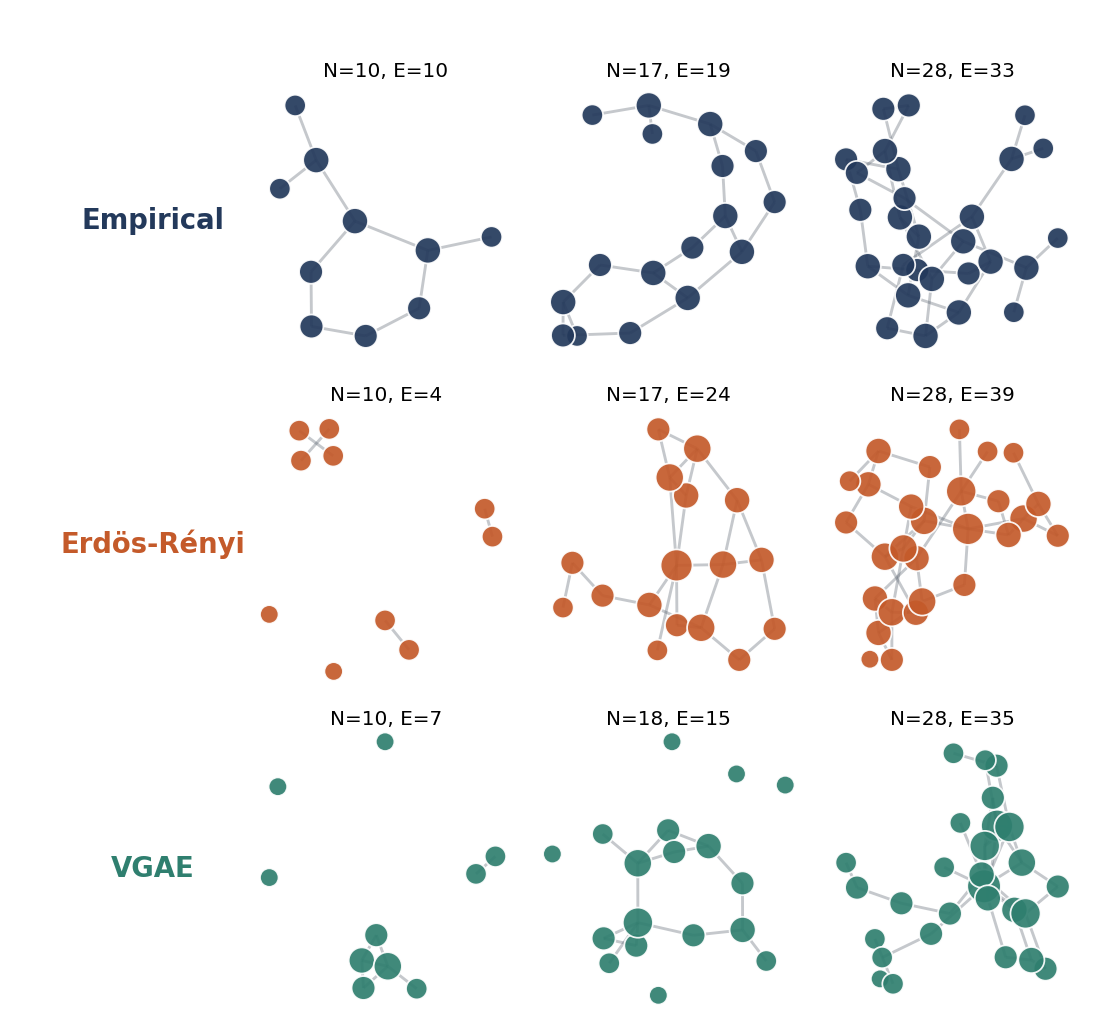
\includegraphics[width=\linewidth,height=0.34\textheight,keepaspectratio]{figures/graph_samples.png}
\caption{Representative samples; node size is degree}
\label{fig:samples}
\end{minipage}\hfill
\hspace{1.1em}
\begin{minipage}{0.55\textwidth}
\centering
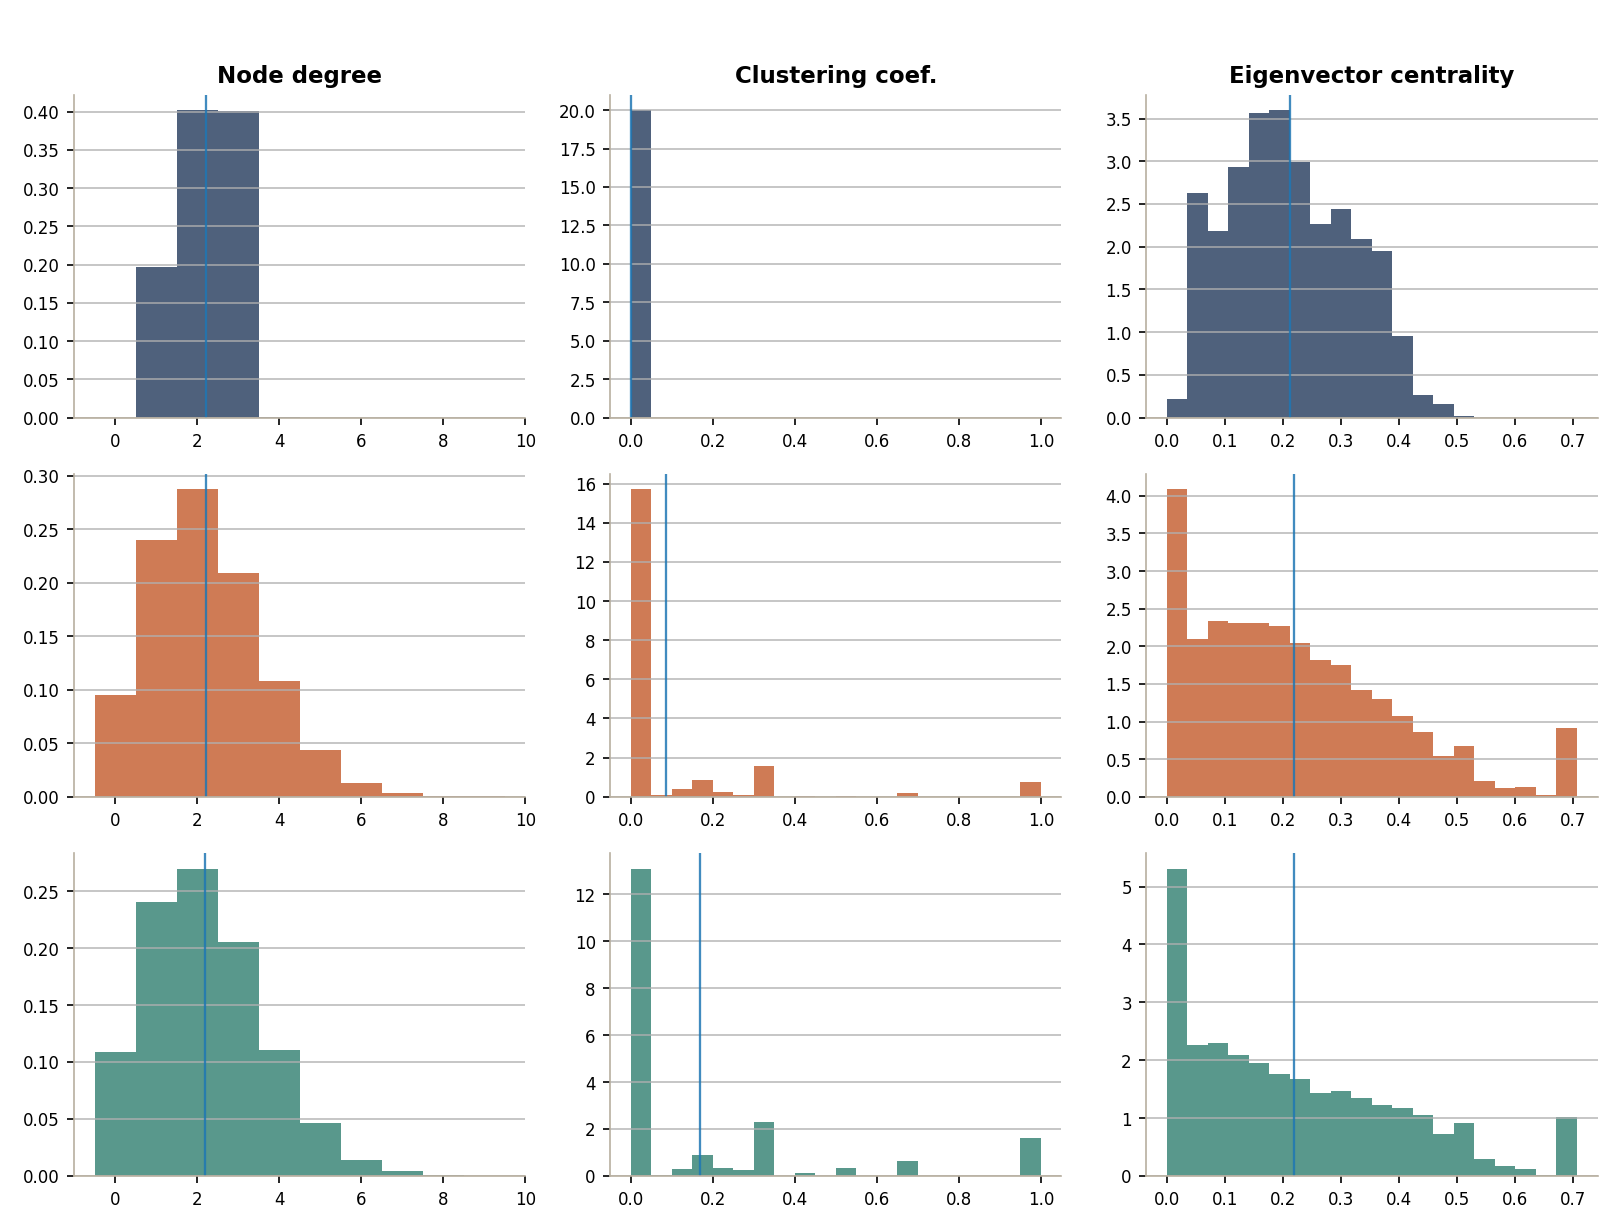
\includegraphics[width=\linewidth,height=0.34\textheight,keepaspectratio]{figures/histograms.png}
\caption{Histograms over 1000 samples (rows top to bottom: empirical, ER, VGAE), shared bins per column}
\label{fig:histograms}
\end{minipage}
\end{figure}

\newpage

\section*{Code snippets}

\subsection*{1. Message passing encoder}

The encoder embeds atom one-hots, runs four rounds of sum-aggregated message passing with residual updates, and emits per-node $(\mu, \log\sigma^2)$ heads.

\begin{lstlisting}[language=Python, caption={GNNEncoder.forward (model.py)}]
def forward(self, x, edge_index):
    num_nodes = x.shape[0]
    state = self.input_net(x)
    for r in range(self.num_rounds):
        message = self.message_net[r](state)
        agg = x.new_zeros((num_nodes, self.state_dim))
        agg = agg.index_add(0, edge_index[1], message[edge_index[0]])
        state = state + self.update_net[r](agg)
    mu = self.mu_head(state)
    logvar = self.logvar_head(state)
    return mu, logvar
\end{lstlisting}

\subsection*{2. Masked VGAE loss}

Padding nodes and self-loops are excluded from both the BCE term (via a pair mask) and the KL term (via the node mask). The BCE is reweighted with \texttt{pos\_weight} to counter the sparsity of MUTAG adjacency matrices.

\begin{lstlisting}[language=Python, caption={vgae\_loss (model.py)}]
def vgae_loss(logits, A, mask, mu_dense, logvar_dense, pos_weight):
    B, N, _ = logits.shape
    pair_mask = (mask.unsqueeze(1) & mask.unsqueeze(2)).float()
    eye = torch.eye(N, device=A.device).unsqueeze(0)
    pair_mask = pair_mask * (1 - eye)
    bce = torch.nn.functional.binary_cross_entropy_with_logits(
        logits, A, pos_weight=pos_weight, reduction='none'
    )
    recon = (bce * pair_mask).sum() / pair_mask.sum()
    node_mask = mask.unsqueeze(-1).float()
    kl_per = -0.5 * (1 + logvar_dense - mu_dense.pow(2) - logvar_dense.exp())
    kl = (kl_per * node_mask).sum() / mask.sum()
    return recon, kl
\end{lstlisting}

\subsection*{3. Sampling and density calibration}

At sample time the inner-product logits are first shifted by $-\log(w_+)$ to undo the BCE reweighting, then a per-graph bisection finds the offset that drives the expected edge count to the empirical density $r_N$ while preserving the decoder's pairwise ranking.

\begin{lstlisting}[language=Python, caption={Bernoulli decode + density shift (model.py)}]
def _decode_bernoulli(self, z, logit_shift=0.0, target_density=None):
    logits = self.decoder(z)[0] + logit_shift
    if target_density is not None:
        logits = logits + density_calibration_shift(logits, target_density)
    probs = torch.sigmoid(logits)
    A = (torch.rand_like(probs) < probs).float()
    A = torch.triu(A, diagonal=1)
    return A + A.t()

def density_calibration_shift(logits, target_density, steps=30):
    n = logits.shape[0]
    rows, cols = torch.triu_indices(n, n, 1, device=logits.device)
    edge_logits = logits[rows, cols]
    target = torch.as_tensor(target_density, device=logits.device).clamp(1e-4, 1 - 1e-4)
    lo = edge_logits.new_tensor(-20.0)
    hi = edge_logits.new_tensor(20.0)
    for _ in range(steps):
        mid = (lo + hi) / 2
        if torch.sigmoid(edge_logits + mid).mean() < target:
            lo = mid
        else:
            hi = mid
    return (lo + hi) / 2
\end{lstlisting}

\subsection*{4. Erdős--Rényi baseline sampler}

The baseline draws $N$ from the empirical size distribution, looks up the density $r_N$ estimated from training graphs of that size, then samples a symmetric Bernoulli upper triangle.

\begin{lstlisting}[language=Python, caption={sample\_baseline (baseline.py)}]
def sample_baseline(num_samples, sizes, probs, densities, seed=0):
    g = torch.Generator().manual_seed(seed)
    graphs = []
    for _ in range(num_samples):
        idx = torch.multinomial(probs, 1, generator=g).item()
        n = int(sizes[idx].item())
        r = densities[n]
        u = torch.rand(n, n, generator=g)
        A = (u < r).float()
        A = torch.triu(A, diagonal=1)
        A = A + A.t()
        graphs.append(adj_to_nx(A))
    return graphs
\end{lstlisting}

\subsection*{5. Training step}

KL is annealed linearly over a 100-epoch warmup, gradients are clipped, and the learning rate decays exponentially. \texttt{pos\_weight} is precomputed once on the training set as the non-edge to edge ratio.

\begin{lstlisting}[language=Python, caption={Training loop core (train.py)}]
num_pos = 0
num_total = 0
for d in train_dataset:
    n = d.num_nodes
    num_pos += d.edge_index.shape[1]
    num_total += n * n - n
pos_weight = torch.tensor((num_total - num_pos) / max(num_pos, 1), device=device)

for epoch in range(epochs):
    beta = beta_max * min(1.0, (epoch + 1) / beta_warmup)
    for data in train_loader:
        data = data.to(device)
        logits, A, mask, mu_d, logvar_d = model(data.x, data.edge_index, data.batch)
        recon, kl = vgae_loss(logits, A, mask, mu_d, logvar_d, pos_weight=pos_weight)
        loss = recon + beta * kl
        optimizer.zero_grad()
        loss.backward()
        torch.nn.utils.clip_grad_norm_(model.parameters(), 5.0)
        optimizer.step()
    scheduler.step()
\end{lstlisting}
\subsection*{6. Weisfeiler--Lehman novelty/uniqueness}

Each generated graph is hashed; novelty compares against training hashes, uniqueness against previously seen samples.

\begin{lstlisting}[language=Python, caption={novelty\_uniqueness (metrics.py)}]
def novelty_uniqueness(samples, train_graphs):
    train_hashes = set(wl_hash(g) for g in train_graphs)
    sample_hashes = [wl_hash(g) for g in samples]
    n = len(samples)
    novel_mask = [h not in train_hashes for h in sample_hashes]
    seen = {}
    unique_mask = []
    for h in sample_hashes:
        if h not in seen:
            seen[h] = True
            unique_mask.append(True)
        else:
            unique_mask.append(False)
    novel = sum(novel_mask) / n
    unique = sum(unique_mask) / n
    novel_unique = sum(a and b for a, b in zip(novel_mask, unique_mask)) / n
    return novel, unique, novel_unique
\end{lstlisting}

\newpage

\begin{description}
\item[What did you use the tool(s) for?] Sanity-checking our derivations (KL term, BCE reweighting, density calibration), debugging tensor-shape mismatches in the message-passing and dense-adjacency code, and reviewing the report for clarity and concision.
\item[At what stage(s) of the process did you use the tool(s)?] During implementation when debugging masking and broadcasting, and during writing to tighten the model description and figure captions.
\item[How did you use or incorporate the generated output?] As a discussion partner. All code, model design choices, and experimental decisions are ours; suggestions from the tool were evaluated and either adopted, modified, or rejected. No generated text was copied verbatim into the report.
\item[Which tool(s) did you use?] Claude Opus 4.7 via the web interface and Claude Code CLI.
\end{description}

\newpage

\bibliography{references}

\end{document}
